\input sys/inputs.tex
\usepackage{pgf,tikz}

\begin{document}

\bigheading{Rozvědka}

% \info{task_name}{infile}{outfile}{points}{timelimit}{memlimit}
% leave this values, if you are not interested
\info{secret}{stdin}{stdout}{100}{2000 ms}{1 GB}

Vojenské rozvědce se podařilo odposlechnout plán nepřátelského vojenského
objektu. Plán objektu je obrázek ve tvaru čtverce tvořený pixely, které mají
vždy buď černou, nebo bílou barvu. Při jeho přenosu byl použit následující
kompresní algoritmus:

\begin{itemize}[nolistsep]

\item Čtverec, který je celý pokrytý jednou barvou, se zakóduje jako jedno
  písmeno -- \texttt{B} v případě černé barvy, nebo \texttt{W} v případě bílé
  barvy.

\item Čtverec, který není celý pokrytý jednou barvou, se rozdělí na čtyři stejně
  velké čtverce. Pro zakódování každého z nich se rekurzivně použije stejný
  algoritmus. Původní čtverec je pak zakódován jako řetězec obalený do kulatých
  závorek, ve kterém jsou postupně zakódovány jednotlivé vnitřní čtverce -- levý
  horní čtverec, pravý horní čtverec, levý dolní čtverec a pravý dolní čtverec.

\end{itemize}

Takto například vypadá obrázek zakódovaný jako \texttt{(B(WWBW)(WBWW)(WWWB))}:

\begin{center}
  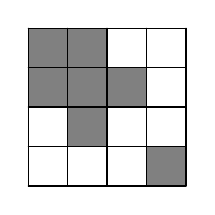
\begin{tikzpicture}[line cap=round,line join=round,x=0.5cm,y=0.5cm]
    \fill[fill=gray] (0,2) -- (1,2) -- (1,3) -- (0,3) -- cycle;
    \fill[fill=gray] (0,3) -- (1,3) -- (1,4) -- (0,4) -- cycle;
    \fill[fill=gray] (1,1) -- (2,1) -- (2,2) -- (1,2) -- cycle;
    \fill[fill=gray] (1,2) -- (2,2) -- (2,3) -- (1,3) -- cycle;
    \fill[fill=gray] (1,3) -- (2,3) -- (2,4) -- (1,4) -- cycle;
    \fill[fill=gray] (2,2) -- (3,2) -- (3,3) -- (2,3) -- cycle;
    \fill[fill=gray] (3,0) -- (4,0) -- (4,1) -- (3,1) -- cycle;

    \foreach \x in {0,...,4}
      \draw [line width=0.5pt,color=black] (\x,0) -- (\x,4);

    \foreach \y in {0,...,4}
      \draw [line width=0.5pt,color=black] (0,\y) -- (4,\y);
  \end{tikzpicture}
\end{center}

Bílá pole jsou volně průchozí. Černě obarvená pole tvoří zdi, takže jimi
procházet nelze. Z bílého pole se dá přejít na jiné bílé pole, pokud s ním má
společnou hranu (nestačí, když se dotýkají pouze rohy).

Rozvědka našla způsob, jak do objektu propašovat svého špiona na určité
souřadnice. Dále se jí podařilo zjistit, na jakých souřadnicích se v objektu
nachází dokumenty s tajnými informacemi, o které má zájem. Od vás by
potřebovala, abyste ověřili, zda se špion dokáže k dokumentům dostat.

\heading{Úloha}

Dostanete plán objektu zkomprimovaný pomocí výše popsaného kompresního
algortimu, souřadnice špiona a souřadnice dokumentů s tajnými informacemi. Špion
i dokumenty se nacházejí na bílých polích. Zjistěte, zda se špion může dostat
k dokumentům pomocí nějaké posloupností bílých polí.

\heading{Vstup}

První řádek vstupu obsahuje číslo $N$: šířku plánu objektu (jedná se o čtverec,
takže výška je stejná jako šířka). Druhý řádek obsahuje řetězec $P$:
zkomprimovaný plán objektu.

Třetí řádek obsahuje čísla $S_x$, $S_y$: číslo sloupce a řádku pole, na kterém
se nachází špion. Čtvrtý řádek obsahuje čísla $D_x$, $D_y$: číslo sloupce a
řádku pole, na kterém se nachází tajné dokumenty.

\bigskip
\noindent
Číslo $N$ je vždy mocninou dvojky. Platí pro něj, že $2 \leq N \leq 2^{60}$.\\
Pro délku řetězce platí $1 \leq \vert P \vert \leq 2 \cdot 10^5$.\\
Pro souřadnice platí, že $1 \leq S_x, S_y, D_x, D_y \leq N$.\\
Pole vlevo nahoře má souřadnice $(1, 1)$. Pole vpravo dole má souřadnice $(N, N)$.\\
Špion se vždy nachází na jiném poli než dokumenty.\\
Ve 20 \% vstupů navíc platí, že $N \leq 1024$.

\heading{Výstup}

Na výstupu vypište jeden řádek se slovem \texttt{POSSIBLE}, pokud se špion může
k dokumentům dostat, nebo se slovem \texttt{IMPOSSIBLE} v opačném případě.

\heading{Příklady}

\sampleIN
4
(B(WWBW)(WBWW)(WWWB))
1 3
3 1
\sampleOUT
POSSIBLE
\sampleEND

\sampleIN
2
(BWWB)
1 2
2 1
\sampleOUT
IMPOSSIBLE
\sampleEND

\end{document}
